\documentclass[fleqn,10pt]{wlscirep}

\usepackage{amsmath}
\usepackage{mathtools}
\usepackage{amssymb}
\usepackage{amsfonts}
\usepackage{graphicx}
\usepackage{epstopdf}

% For the debug usage only
\usepackage{color}

\DeclarePairedDelimiter\bra{\langle}{\rvert}
\DeclarePairedDelimiter\ket{\lvert}{\rangle}

% For the debug usage only
\newcommand{\red}{\color{red}}
\newcommand{\blue}{\color{blue}}

% Elliptic functions
\newcommand{\sn}{\textrm{sn}}
\newcommand{\cn}{\textrm{cn}}
\newcommand{\dn}{\textrm{dn}}
\newcommand{\sd}{\textrm{sd}}
\newcommand{\cd}{\textrm{cd}}
\newcommand{\nd}{\textrm{nd}}
\newcommand{\am}{\textrm{am}}

% Title and authors
\title{Exciton-polariton Josephson junctions at finite temperatures}

\author[1]{M. E. Lebedev}
\author[1]{D. A. Dolinina}
\author[2]{Kuo-Bin Hong}
\author[2]{Tien-Chang Lu}
\author[3, 4, 5]{A. V. Kavokin}
\author[1, 6, *]{A. P. Alodjants}

\affil[1]{ITMO University, St. Petersburg 197101, Russia}
\affil[2]{Department of Photonics, National Chiao Tung University, Hsinchu 300, Taiwan}
\affil[3]{Spin Optics Laboratory, St. Petersburg State University, Ul’anovskaya, Peterhof, St. Petersburg 198504, Russia}
\affil[4]{School of Physics and Astronomy, University of Southampton, SO17 1BJ Southampton, United Kingdom}
\affil[5]{Istituto CNR-SPIN, Viale del Politecnico 1, I-00133, Rome, Italy}
\affil[6]{Vladimir State University named after A. G. and N. G. Stoletovs, Gorkii Street 87, Vladimir, Russia}

\affil[*]{alexander\_ap@list.ru}

% \keywords{\dots}

\begin{abstract}

We consider finite temperature effects in a non-standard Bose-Hubbard model for an exciton polariton Josephson junction (EPJJ) that is characterised by complicated potential energy landscapes (PEL) consisting of sets of barriers and wells.
We show that the transition between  thermal  activation (classical) and tunneling (quantum) regimes exhibits universal features of the first and second order phase transition (PT) depending on the PEL for two polariton condensates.
In the presence of dissipation the relative phase of two condensates exhibits non-equilibrium PT from the quantum regime characterized by efficient tunneling of polaritons to the regime of permanent Josephson or Rabi oscillations, where the tunneling is suppressed, respectively.
This analysis paves way for the application of coupled polariton condensates for the realisation of a quantum annealing algorithm.
 
\end{abstract}

\begin{document}

\flushbottom
\maketitle

% (?)
\thispagestyle{empty}

\section*{Introduction}

In the XXI century, the studies of exciton-polariton Bose-Einstein condensates (BEC) in various type of semiconductor microstructures have become an important area of research in photonics and semiconductor physics, see e.g. \cite{Sanvitto, Guillet}.
Microcavity exciton polaritons are bosonic quasiparticles representing admixtures of quantized cavity photons and quantum well excitons.
Semiconductor microcavities are promising for various optoelectronic applications where the quantum  matter-field interface plays a crucial role.
In particular, it is worth to mention experimental demonstrations of polariton lasers with electrical injection \cite{Bhattacharya,Schneider}, polariton amplifiers \cite{Niemietz}, switches \cite{Amo_2010}, transistors \cite{Ballarini}, polariton circuits and optical logic elements \cite{Sturm,Liew}.
Although exciton polariton condensates exhibit the Bose-Einstein statistics above the lasing threshold and are characterized by a macroscopic occupation of the ground state at certain pumping rate that is less than the threshold pumping for convenient lasers, they are not in a true thermodynamic equilibrium state \cite{Byrnes_2014,Sun}. Non-equilibrium features of exciton polariton condensates play an important role in various manifestations of their collective (many body) states such as superfluidity \cite{Carusotto_2013,Amo_2009}, quantized vortices \cite{Lagoudakis_2008,Lagoudakis_2009}, soliton formation \cite{Sich}, Josephson oscillations and macroscopic self-trapping \cite{Abbarchi,Lagoudakis_2010}.
    
The problem of distinguishability of statistically classical (thermal) and quantum regimes for exciton polariton condensates is very important for their possible applications in quantum information technologies, see e.g. \cite{Dominici}.
Fast switching properties (the typical switching time of a few picoseconds), relatively strong nonlinear response and flexibility to external optical and/or electrical pumping spin degrees of freedom made microcavity polaritons potentially promising for quantum computation and quantum information processing, see, e.g. \cite{Demirchyan,Pagel,Kyriienko,Solnyshkov_2015, Dominici}.

Here we specifically focus on the quantum annealing problem that is relevant to the searching algorithm for the global minimum of the potential energy landscape (PEL) consisting of a set of barriers and wells, see e.g.  \cite{Santoro, Das}.
In a purely classical  (thermal) regime the {bosonic quasipartcles cross barriers stochastically} at finite temperature with the help of thermal activation process if the thermal energy is large enough, see Fig. \ref{pic:potential_picture}. Contrary, in a quantum limit the same system undergoes quantum tunneling through the barrier. Obviously, the shape (height and thickness) of the barrier plays an essential role in this case \cite{Das, Lewenstein}. It has been shown recently in \cite{Lewenstein} that the annealing algorithm relies in general case on the combination of thermal annealing and quantum tunneling. The     
collective (bosonic) character of polariton condensation could be used for the acceleration of the physical implementation of the search algorithm \cite{Yan}. The authors of Refs. \cite{Lago1, Lago2} propose polariton graphs as an analog platform for minimizing the XY -- Hamiltonian by exploring the non-equilibrium character of exciton polariton condensates and mimicking various magnetic phases with them.  An original technique of nonresonant spatially  modulated pumping beam  have been used to imprint two-dimensional polariton graphs with different topology and different heights of potential barriers. Importantly, the phase-locking  between arbitrary neighboring vertices might be practically achieved in this case.
%
\begin{figure}[ht]
\center{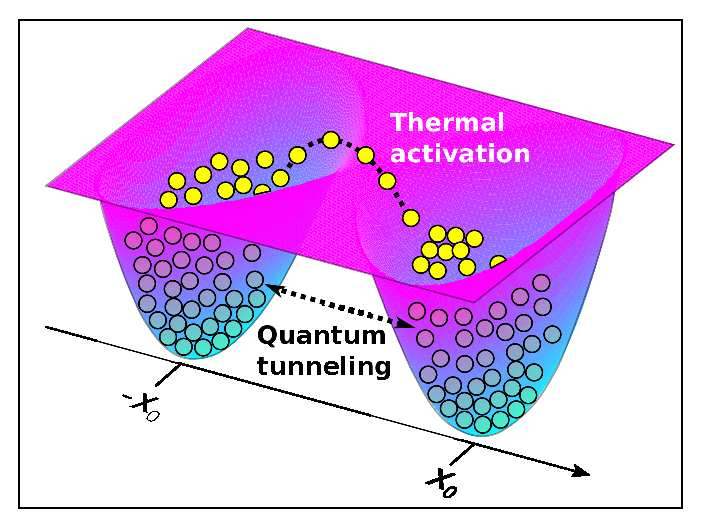
\includegraphics[width=0.5\linewidth]{pic/potential_picture.eps}}
\caption{Scketch of two tunnel coupled exciton condensates. The two minima of the trapping potential $U$ are situated in the points $+x_0$ and $-x_0$. At thermal equilibrium the interplay between thermal and quantum annealing effects is governed by the blue shift of condensates, effective temperature of exciton-polaritons and the shape of the potential. \label{pic:potential_picture}}
\end{figure} 
%

In the present paper we study the effect of a finite effective temperature on the coupling of quasi-equilibrium exciton-polariton condensates accounting for the competing thremal and quantum annealing effects.  
Recently Yongbao Sun et al \cite{Snoke_2017} reported the observation of a quasi-equilibrium low branch exciton polariton condensate in a high Q-factor microcavity characterised by a remarkably long photon lifetime of $135ps$.
Clearly, exciton polaritons with long lifetime are promising candidates for quantum technologies \cite{Demirchyan}.
One of the crucial advantages of exciton-polaritons over cold atoms consists in a perspective of room temperature operation of polariton devices.
In this context, it is very important to reveal the impact of temperature on the physics of interacting polariton condensates.
It should be also noted that the effective temperature of a polariton gas may be introduced in the quasi-equilibrium approximation, which is not necessarily valid in all cases but constitutes an important starting point of any analysis. Further steps would involve a full kinetic modelling for a non-equilibrium polariton gas.  
 
To be specific, here we consider an exciton polariton Josephson junction (EPJJ).
We study the interplay of two mechanisms of coupling between the condensates in order to reveal the cross-over from the quantum tunneling to the incoherent coupling regime that may occur at finite temperatures \cite{Aleiner, Shelykh_2008, Borgh_2010}. 
In particular, we are interested in a generic problem of the quantum-classical phase transition (PT) applied to two-level (spin) systems \cite{Chudnovsky_1997, Caldeira, Larkin, Riseborough, Zhang, Owerre}.
Traditionally,  studies in this field are limited by consideration of superconductor devices \cite{Ankerhold} where macroscopic quantum tunneling phenomena plays an essential role.
In particular, it is worth to mention here the Schr\"odinger cat state formation \cite{Leggett} and the 	design of quantum gates with superconductor qubits for quantum computing where a macroscopic quantum coherence for the phase is important \cite{Makhlin}.
  
We shall consider a generalised model of EPJJ that relates to so-called non-standard Bose-Hubbard models (see \cite{Dutta} and references therein) where the energy of polariton-polariton scattering contributes to the tunneling parameter matrix elements \cite{Aleiner, Shelykh_2008, Borgh_2010, Solnyshkov_2008, Sarchi}.
In particularly, we pay attention to the temperature dependent quantum critical phenomena occurring in the presence of macroscopic tunneling.
We aim at the formulating of the criteria for realisation of the quantum tunneling regime that is crucial for the realisation of the quantum annealing algorithms and exciton-polariton quantum gates.

This paper is organised as follows.
In Sec. \ref{sec:quantum_phase} we introduce the quantum phase model for EPJJ and discuss various regimes of coupling between two condensates at zero temperature and in the limit of an infinite exciton polariton lifetime.
Section \ref{sec:quantum_classical} presents the results obtained for a quantum-classical PT problem and addresses the quantum phase at finite temperatures.
The influence of non-equilibrium effects involving the microcavity exciton polaritons possessing a finite lifetime is discussed in Sec. \ref{sec:non-equilibrium}.      
In Conclusion, we summarize the obtained results.
In the Supplementary Material we explain in details the extended model of EPJJ formulated within the tight-binding approximation.
 
\section*{Results} 
 
\subsection*{The Quantum Phase Model \label{sec:quantum_phase}}

We consider a system of two spinless exciton-polariton condensates localised in lateral potential traps created in a planar semiconductor microcavity.
The condensates are confined by a W-shape potential $U(x)$ possessing two minima at the points $\pm x_0$, see Fig. \ref{pic:potential_picture}.
Polaritons are pumped to the condensates from a reservoir of incoherent excitons. In this and next Section, we shall neglect the finite polariton lifetime and assume that the polariton gas is at the thermal equilibrium.   
We account for the polariton-polariton repulsion.

We shall use the pseudo-spin operator representation for the Hamiltonian describing our EPJJ model system that has a form (the details of the model are presented in the Supplementary Material): 
%
\begin{equation}
\hat{H} = \alpha \hat{S}_z^2 + \beta \hat{S}_x^2 - B \hat{S}_x.
\label{eq:hamiltonian_spin}
\end{equation}
%
The coefficients in Eq. (1) characterize the tunnel coupling of two trapped condensates:
the parameters $\alpha$ and $\beta$ are proportional to the overlap integrals of real symmetric ($\Phi_+$) and antisimmetric ($\Phi_-$) wavefunctions of two condensates that are
$\int \Phi_i^2 \Phi_j^2 dx, i,j \in \{+,-\}$, $B$ is determined by difference of chemical potentials which obey stationary Gross-Pitaevskii (GP) equations for two trapped condensates.

It is important to note that the last term in Eq. (1) characterizes the familiar XY--model Hamiltonian  considered in
\cite{Lago1, Lago2}.
The second term in (1) introduces an additional part that has no analogy in the XY-Hamiltonian; it is proportional to $\cos(2\phi)$, where $\phi$ is the phase difference between two polariton condensates.
We will show that this term becomes essential if the barrier separating two condensates is sufficiently large.
It is convenient to introduce the pseudo-spin operators in a form
% 
\begin{subequations}
\begin{align}
\hat{S}_x = & s \cos{\phi} - \sin{\phi} \dfrac{d}{d \phi}, \\
\quad \hat{S}_y = & s \sin{\phi} + \cos{\phi} \dfrac{d}{d \phi}, \\
\hat{S}_z = & -i\dfrac{d}{d \phi},
\end{align}
\label{eq:pseudo_spin_diff}
\end{subequations}
%
The operators defined in Eq. (\ref{eq:pseudo_spin_diff}) obey familiar $SU(2)$ algebra commutation relations $[\hat{S}_i, \hat{S}_j] = i\epsilon_{ijk}\hat{S}_k,  i,j,k=x,y,z$.
After some straightforward calculations from (\ref{eq:hamiltonian_spin}) one can obtain
%
\begin{equation}
\begin{array}{lcl}
H & = & -(\alpha - \beta \sin^2 \phi) \dfrac{d^2}{d \phi^2} - (\beta(s-\dfrac{1}{2})\sin{2\phi} - B\sin{\phi}) \dfrac{d}{d \phi} \\
&& - Bs \cos \phi - \beta s^2 \sin^2 \phi - \beta s \cos^2 \phi.
\end{array}
\label{eq:hamiltinian_s}
\end{equation}
%
Thereafter we assume that both condensates are composed by macroscopically large numbers of particles, i.e. the $s = N/2 >> 1$ is C - number.
The general stationary Schroedinger equation with a Hamiltonian (\ref{eq:hamiltinian_s}) writes:
%
\begin{equation}
\begin{array}{l}
(\alpha - \beta \sin^2 \phi) \dfrac{d^2 \Phi}{d \phi^2} + (\beta s\sin{2\phi}-B\sin{\phi})) \dfrac{d \Phi}{d \phi} \\
+ (E + B s \cos \phi + \beta s^2 \sin^2 \phi) \Phi = 0,
\end{array}
\label{eq:schrodinger}
\end{equation}
%
where $\Phi \equiv \Phi(\phi)$ is some $2\pi$-periodic wavefunction that characterizes quantum phase properties \cite{Anglin}.
It is possible to eliminate the term with first derivative in Eq. (\ref{eq:schrodinger}).
In order to find the explicite form of the function $\Phi$, it is convenient to substitute it by:
%
\begin{equation}
\Phi(\phi) = \Psi(z) \exp \Big( s \ln \dn{z} - \dfrac{\Lambda s}{2 \sqrt{\lambda (1 - \lambda)}} \arctan \Big( \sqrt{\dfrac{\lambda}{1 - \lambda}} \cn{z} \Big) \Big),
\label{eq:transformation_of_phi}
\end{equation}
%
where $z = \int \limits_0^\phi \dfrac{d \xi}{\sqrt{1 - \lambda \sin^2 \xi}} = F(\phi, \lambda)$ is a new phase variable; $F(\phi, \lambda)$ is the incomplete elliptic integral of the first kind.
In (\ref{eq:transformation_of_phi}) we have introduced dimension-less parameters $\Lambda = \dfrac{B}{\alpha s}$, $\lambda = \dfrac{\beta}{\alpha}$.
Inserting (\ref{eq:transformation_of_phi}) into (\ref{eq:schrodinger}) we arrive to the familiar form of a Schr\"odinger equation
% 
\begin{equation}
\alpha \frac{d^2\Psi}{dz^2} + (E - V(z))\Psi = 0.
\label{eq:schrodinger_usual}
\end{equation}
%
This equation describes an effective particle with the mass  $m = \dfrac{\hbar^2}{2 \alpha}$ and energy $E$, that is confined by the potential $V(z) = \alpha s^2 V_0(z)$ with
%
\begin{equation}
V_0(z) = \frac{ (\frac{1}{4} \Lambda^2 - \lambda (1 - \lambda)) \sn^2{z} - \Lambda \cn{z}}{\dn^2{z}}.
\label{eq:potential}
\end{equation}
%

The dependences of the trapping potential $V_0(z)$ on the phase variable $z$ are shown in Fig. \ref{pic:phase_potential}. The period of the functions is  $4K(\lambda)$.
The dependence of the $\lambda$ parameter on normalized half of the inter-well distance $\dfrac{x_0}{a}$ can be approximated by $\lambda = 0.5 \Big( \exp \Big[ \dfrac{2 x_0^2}{a^2} \Big] - 1 \Big)^{-1}$ by using variational approach,  see Suppl. Materials.
The well-known behaviour of the quantum phase mesoscopic Josephson junction (that map to the XY--model, \cite{Lago1, Lago2} ) can be recovered from (\ref{eq:hamiltonian_spin}), (\ref{eq:potential}) at $\lambda = 0$ and shown by red curves in Fig. \ref{pic:phase_potential}. This limit corresponds to  infinitely large inter-well distances, with $x_0 \to \infty$.
On the other hand, the $\lambda$ -- parameter exhibits a sharp increase at $\dfrac{x_0}{a} \ll 1$.
Obviously, in this limit our EPJJ model based on the assumption of a relatively weak coupling between trapped condensates breaks down.
Below we are focusing on $\lambda$ -- parameters which belong to the range of $0 < \lambda < 1$ and correspond to the moderate values of $\dfrac{x_0}{a}$ such as $\dfrac{x_0}{a} \geq 0.45$. 
%
\begin{figure}[ht]
\begin{center}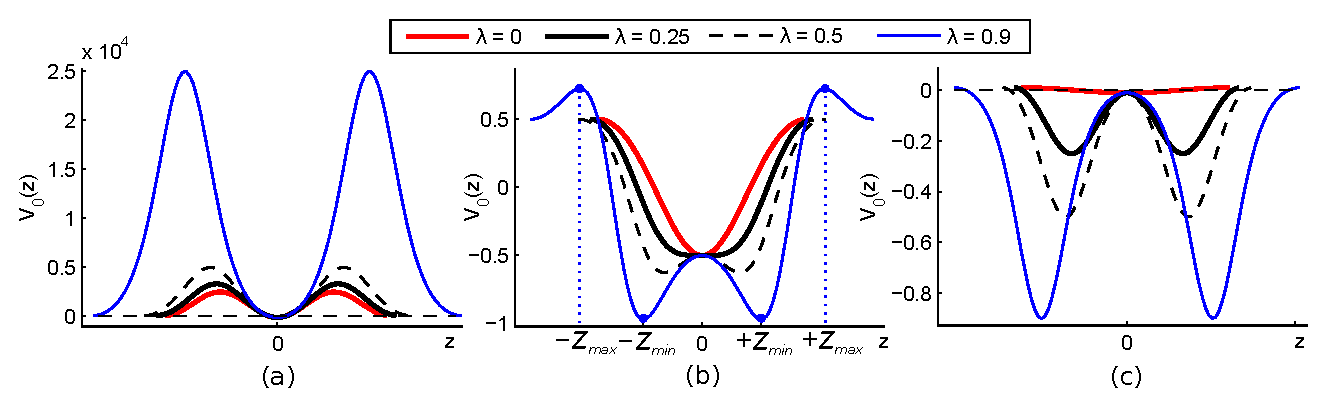
\includegraphics[width=1\linewidth]{pic/potentials.eps}
\end{center}
\caption{
Effective dimension-less potential $V_0(z)$ for (a) $\Lambda = 100$, (b) $\Lambda = 0.5$ , and (c) $\Lambda = 0.01$ as a function of the elliptic integral phase coordinate $z$.
Points $\pm z_{min}$ and $\pm z_{max}$ in (b) correspond to global minima and maxima of the potential, respectively; $E$ is the energy of the particle that experiences either quantum tunneling or thermal activation, see Section \ref{sec:quantum_classical}.
\label{pic:phase_potential}}
\end{figure}
%
The analysis of the quantum phase can be performed in three domains determined by vital $\Lambda$--parameter values, \cite{Anglin}.

\textit{Rabi regime} $\Lambda \gg 1$. In this limit the trapping potential can be approximated by $V_R(z) = \dfrac{1}{4} \Lambda^2 \sd^2{z}$.
Physically, for any value of $\lambda$ -- parameter belonging to the domain 0$<\lambda <1$ the system exhibits (Rabi) oscillations for the phase.
In particular, small amplitude oscillations which are inherent to familiar Rabi regime can be achieved for negligable $\lambda$ --- see Fig. \ref{pic:phase_potential}a and \cite{Anglin}.

\textit{Fock regime} $\Lambda \ll 1/N^2$.
In purely quantum limit $\Phi(\phi) \to (2\pi)^{-1/2}$.
In this regime, when inequality $\Lambda \ll \lambda < 1$ is held, Eq.(\ref{eq:schrodinger_usual}) transforms to the Mathieu equation that is characterised by the set of eignen states consisting of all Mathieu functions.

\textit{Josephson regime} $1/N^2\ll\Lambda <1$.
This regime corresponds to the intermediate case between Rabi and Fock limits --- see Fig. \ref{pic:phase_potential}b.
The behavior of the phase depends on the ratio between the parameters $\Lambda$ and $\lambda$.
If $\Lambda \ge 2\lambda$ the potential $V_0(z)$ possesses only one minimum at $z = 0$ and $V(0) = -\Lambda$. 

In the opposite limit, for $\Lambda < 2 \lambda$, the effective quantum ``particle'' described by Eq. (\ref{eq:schrodinger_usual}) is trapped at the two minima of $V_0(z)$ that correspond to the $W$ -- like potential with coordinates $z_{min} = \pm \cn^{-1}{\frac{\Lambda}{2 \lambda}}$ and appearing for both of Josephson and Fock regimes, see Fig. \ref{pic:phase_potential}b,c.  
The depth of the potential minima depends on the $\lambda$ parameter.
It is interesting to note that for $\Lambda > 2(1 - \lambda)$ the potential $V_0(z)$ possesses a local minimum at $\pm 2 K(\lambda)$, see Fig. \ref{pic:potential_picture}b.

\subsection*{Annealing problem versus Quantum-classical PT's \label{sec:quantum_classical}}

Experimentally, exciton-polariton condensates are being observed at elevated temperatures, up to the room temperature in wide-gap semiconductor microcavities \cite{Sanvitto,Guillet}.
At high temperatures the validity of the quantum coherent treatment of the Josephson problem is limited.
In this section, we study the limits of validity of the quantum approach which also set the limits of the system suitability for quantum annealing \cite{Das}.

To be more specific we consider the tunneling in an effective $W$ -- like potential shown in Fig. \ref{pic:phase_potential}b. We assume the thremal equilibrium condition to be fulfilled for an ensamble of exciton-polaritons at finite temperatures $T$, that would correspond to a hypothetic case of polaritons with the infinite life-time.  We note in this connection that in the recent experiments \cite{Snoke_2017} the measured polariton lifetime was as long as $275ps$, which would be sufficient to justify the above approximation.

A transition between two stable states (say, between points $-z_{min}$ and $+z_{min}$ in Fig. \ref{pic:phase_potential}b) can happen  either through the quantum tunneling or, in classical way, due to the thermal activation. 
Obviously, at high temperatures such as $k_{B}T\ge\Delta V$ ($\Delta V$ is the height of the barrier between two states with minimum of potential energy) the particle jumps over the barrier governed by the thermoactivation (Arrhenius) escape rate $\Gamma \sim e^{-\Delta V /k_{B}T}$ \cite{Larkin}. This process is inherent to the classical (thermal) annealing problem \cite{Das}. 
In the ``low temperature'' limit $k_{B}T\ll\Delta V$ polaritons undergo quantum tunneling through the barrier with a vanishing rate, that excludes realisation of the quantum annealing scheme.

Our description is based on imaginary time path integral approach \cite{Ankerhold}.
The imaginary-time action obtained within the WKB method approaches as $S(E) = \oint (\tfrac{1}{2} m \dot{z}^2 + V(z)) d \tau$.
The decay rate $\Gamma \sim e^{-S_{min}/\hbar}$ in our approach can be expressed through the minimal value $S_{min}$ of the action.
The trajectories which minimize the action $S_T$ obey the classical equation of motion $m \ddot{z} = \frac{d V}{dz}$ written for the thermon ``particle'' that oscillates within the inverted potential $-V(z)$.
Periodic solutions of this equation satisfy
%
\begin{equation}
\tfrac{1}{2} m \dot{z}^2 = V(z) - E(\tau_p),
\label{eq:total_energy}
\end{equation}
%
where $\tau_p = \hbar / k_B T$ is a thermon period corresponding to the energy $E(\tau_p)$ and shown in Fig. \ref{pic:phase_potential}b;
%
\begin{equation}
\tau_p(E) = \sqrt{2 m} \int_{z_1(E)}^{z_2(E)} \frac{dz}{\sqrt{V(z) - E}}.
\label{eq:thermon_period}
\end{equation}
%
In (\ref{eq:thermon_period}) the $z_{1,2}(E)$ are the turning points, see Fig. \ref{pic:phase_potential}b.
Eqs.(\ref{eq:total_energy}),(\ref{eq:thermon_period}) taken at the energy $E = 0$ and temperature $T = 0$ characterize the instanton solution with an infinite period.
Combining the equation for $S(E)$ 
%(\ref{eq:thermon_action_1}) 
with (\ref{eq:total_energy}) we arrive to 
%
\begin{equation}
S_T = 2 \sqrt{2 m} \int_{z_1(E)}^{z_2(E)} \sqrt{V(z) - E} ~dz + E \tau_p (E).
\label{eq:thermon_action_2}
\end{equation}
%

To reveal the thermodynamic properties of the system it is necessary to consider the small amplitude oscillations at the bottom, $z=0$, of the inverted potential $-V(z)$.
The action in this case reads: 
%
\begin{equation}
S_0 = \Delta V \tau_p (E).
\label{eq:thermal_action}
\end{equation}
%
The expansion of the potential $V(z)$ into a series and excluding the constant value $V(0)$ gives:
%
\begin{equation}
\begin{array}{lcl}
V(z) & = & \alpha s^2 \Big[ \left( \frac{1}{4} \Lambda^2  - \frac{2\lambda - 1}{2} \Lambda - \lambda (1 - \lambda) \right) z^2 \\
&& + \left( \frac{2\lambda - 1}{12} \Lambda^2 - \frac{16\lambda^2 - 16\lambda + 1}{24} \Lambda - \frac{\lambda (1 - \lambda) (2\lambda - 1)}{3} \right) z^4 + o(z^4) \Big].
\end{array}
\label{eq:potential_teylor}
\end{equation}
%
In particular, if the inverted potential $-V(z)$ has the form $z^2 - z^4$ the second order phase transition occurs.
If $-V(z)$ behaves as $z^2 + z^4$ the first order phase transition take place.
The phase boundary between the 1st and 2nd order phase transitions is determined by the relation
%
\begin{equation}
\Lambda = \frac{1 - 16\lambda + 16\lambda^2 + \sqrt{1 + 32\lambda - 32\lambda^2}}{4(2\lambda - 1)}.
\label{eq:order_border}
\end{equation}
%

We summarize our results in Fig. \ref{pic:phase_boundary_combined}. An inset demonstrates various types of  phase potentials $V_0(z)$ inherent to our EPJJ model. The first order PT occurs for two type of potentials in the shaded region bounded by bold  (red) curve.  Second order PT's appear for the potential landscapes taken from the dark area. 
%
\begin{figure}[ht]
\center{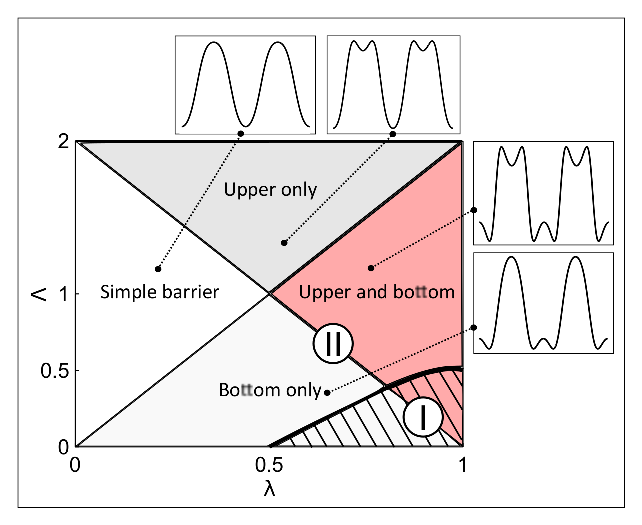
\includegraphics[width=0.5\linewidth]{pic/phase_transition_diagram_combined.eps}}
\caption{Diagram of the phase boundary for the 1st- and 2nd-order PT's in $\Lambda$, $\lambda$ -- parameters plane.
The potential energy landscapes (PEL's) are shown in the windows. \label{pic:phase_boundary_combined}}
\end{figure}
%

The crossover temperature $T_{c}^{(2)} = \hbar \omega_0/ 2 \pi k_B$ of 2nd-order PT transition  is 
%
\begin{equation}
T_{c}^{(2)} = T_{0} \sqrt{\lambda (1 - \lambda) + (2 \lambda - 1) \tfrac{\Lambda}{2} - \tfrac{1}{4} \Lambda^2},
\label{eq:second_order}
\end{equation}
%
where  $\omega_0 = \frac{2 \alpha s}{\hbar} \sqrt{\lambda (1 - \lambda) + \tfrac{1}{2} (2 \lambda - 1) \Lambda - \tfrac{1}{4} \Lambda^2}$ is a frequency of small oscillations of the thermon ``particle'' near the bottom of inverted potential,  $T_{0}=\alpha N / 2\pi k_B$ is a characteristic temperature that inherent to exciton polariton system.  The $T_{0}$  implies important time scale $\tau_0=2\pi\hbar/ \alpha N$ that can be understood as thermon particle ``lifetime''. Notably, as it is follows from (\ref{eq:second_order}) there is no barrier at $z = 0$ for $\Lambda \ge 2\lambda$ -- see the white domain in Fig. \ref{pic:phase_boundary_combined}.
 
In Fig. \ref{pic:action_period}a we represent the results exhibiting 1st-order PT inherent to narrow shadow domain in Fig. \ref{pic:phase_boundary_combined} where discontinuity of the derivative $dS / dT$ occurs.
It is clearly seen that the first derivative of $S_{min}$ is discontinuous in this case and the dependence of the normalized thermon period  $\tau_p / \tau_0$ on the energy $E$ is non-monotonic, see the inset in Fig. \ref{pic:action_period}a.
The critical temperature $T_{c}^{(1)}$ belongs to the temperature domain $T_{min} < T_{c}^{(1)} < T_{max}$ and it can be found out numerically by solving Eqs.(\ref{eq:thermon_period}) - (\ref{eq:thermal_action}) in the particular case of $S_T = S_0$.
 
Analytically, the critical temperature $T_{c}^{(1)}$ may be estimated from $T_{c}^{(1)} = \Delta V / S_{inst}$, where $S_{inst}$ is an instanton action that can be represented as $S_{inst} = S(E_{min})$.
After some straightforward calculations for $B$ we obtain
%
\begin{equation}
\begin{array}{c}
S_{inst} = S(E_{min}) = 2 s \hbar \left[ \ln \frac{2 \sqrt{\lambda} + \sqrt{4 \lambda^2 - \Lambda^2}}{2 \sqrt{\lambda} - \sqrt{4 \lambda^2 - \Lambda^2}} - \frac{\Lambda}{\sqrt{\lambda (1 - \lambda)}} \arctan \left( \frac{\sqrt{(1 - \lambda) (4 \lambda^2 - \Lambda^2)}}{\Lambda} \right) \right].
\end{array}
\label{eq:B_action}
\end{equation}
%

%
\begin{figure}[ht]
\begin{minipage}[h]{0.49\linewidth}
\center{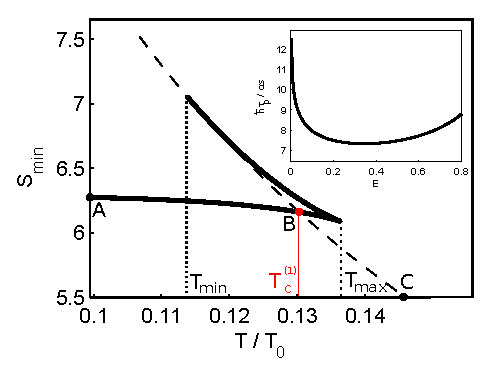
\includegraphics[width=1\linewidth]{pic/action_period_1st_order_transition.eps} \\ (a)}
\end{minipage}
\hfill
\begin{minipage}[h]{0.49\linewidth}
\center{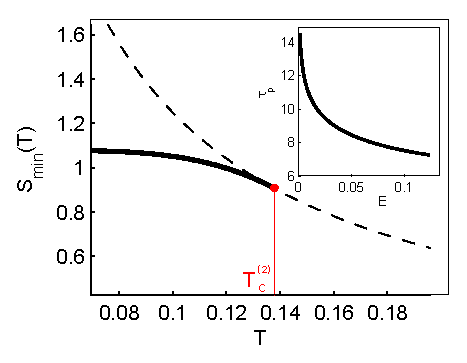
\includegraphics[width=1\linewidth]{pic/action_period_2nd_order_transition.eps} \\ (b)}
\end{minipage}
\caption{Dependences of the minimal action $S_{min}$ (ABC-(blue) curve) taken in $s\hbar$ units as a function of the normalized temperature $ T/T_{0}$ for (a) 1st-order PT, $\lambda = 0.9$, $\Lambda = 0.1$; and, (b) 2nd-order PT, $\lambda = 0.5$, $\Lambda = 0.5$; the solid (bold) line corresponds to the thermon action, $S_T$; the dashed line corresponds to the thermodynamic action, $S_0 = \hbar \Delta V / k_B T$, $S_{min} = \min \{S_0, S_T\}$. The inset shows the dependences of normalized thermon period $\tau_p / \tau_0$ on energy $E$ expressed in $\alpha s^2$ units. 
\label{pic:action_period}}
\end{figure}
%

Figure \ref{pic:action_period}b displays 2nd-order PT from quantum (solid bold line of $S_T$) to thermal (classical) regimes --- dashed bold line of $S_0$.
The crossover occurs at the critical temperature $T_{c}^{(2)}$ where $S_T = S_0$ and {$E = E_0$}.
The inset demonstrates a monotonic dependence of normalized thermon period $\tau_p/\tau_0$ on energy $E$ that is inherent to second-order phase transition.
Closest to the critical point with energy $E=E_0$ the thermon undergoes small amplitude oscillations.

The connection with phenomenological Landau theory of phase transitions  (cf. \cite{Lif}) can be obtained by introducing the ``order parameter'' $P$ that is  (cf. [34]).
%
\begin{equation}
P = \sqrt{\dfrac{V(0) - E}{\Delta V}}.
\label{eq:p_parameter}
\end{equation}
%

Physically, $P$ -- parameter describes  seminal features of potential shape for the ``particle'' possessing energy $E$ -- see Fig. \ref{pic:phase_potential}b.
Figure \ref{pic:p_parameter} shows the behaviour of the introduced order parameter.
One can see that the phases corresponding to the quantum tunneling and classical thermal activations are separated by the second order phase transition.

%
\begin{figure}[ht]
\center{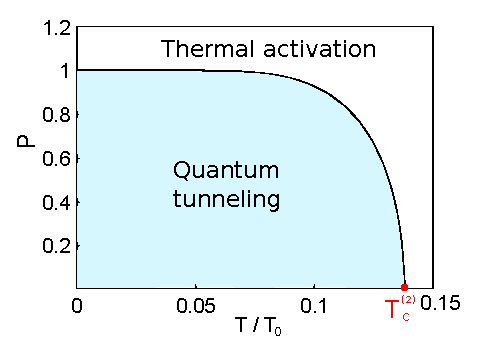
\includegraphics[width=0.5\linewidth]{pic/p_parameter.eps}}
\caption
{The dependence of the $P$ -- parameter on the normalized temperature $T/T_{0}$.  The parameters $\lambda$, $\Lambda$ are the same as in Fig. \ref{pic:action_period}b.
\label{pic:p_parameter}}
\end{figure}
%
In the optical experiments one usually has a better control of the exciton-polariton density than their effective temperature, see e.g. \cite{Sanvitto,Guillet}.
For instance, the density of polariton gas can be changed by varying the optical pump intensity.
In Fig. \ref{pic:temperatures} we plot a numerically calculated critical temperature of the 1st and 2nd order PTs as a function of the $\Lambda$-parameter for experimentally accessible semiconductor Josephson junction samples.
The bold (green) line corresponds to the analytical solution obtained with  Eq. (\ref{eq:B_action}).
Since the $\Lambda$-parameter is inversely proportional to the density of the exciton polariton gas (and the blue-shift of the energy of the corresponding photoluminescence peak) Fig. \ref{pic:temperatures} establishes an important relation between the critical temperatures discussed in the paper and the relevant exciton polariton densities.
%
\begin{figure}[ht]
\center{\includegraphics[width=0.5\linewidth]{pic/phase_transition_temperatures.eps}}
\caption
{The dependence of the normalized critical temperature $T_{c}/T_{0}$ as a function of the parameter $\Lambda$. The bold (green) line corresponds to the analytical expression for  $T_{c}^{(1)}$ given by Eq. (\ref{eq:B_action}).
\label{pic:temperatures}}
\end{figure}
%

Now let us consider the decay of the state of the system that corresponds to the upper minimum of the potential $V(z)$ located at $\pm 2K(\lambda)$ in Fig. \ref{pic:phase_potential}b and exists for $\Lambda > 2(1 - \lambda)$.
Physically, the decay takes place because of the tunneling of our effective particle through the barrier located at one of the points $z_{max} = \pm \cn^{-1} \left( -\frac{2(1 - \lambda)}{\Lambda} \right)$.
By expanding the potential $V(z)$ in the vicinity of $z_{max}$ it is possible to show that only the 2nd-order PT with a temperature $T_{c}^{(2)} = (T_{0}/ 2) \sqrt{\frac{\Lambda^2}{1 - \lambda} - 4(1 - \lambda)}$ may take place in this case.

Let us briefly discuss methods of the experimental study of the quantum-classical PT for the polariton Josephson junctions.
Our estimations show that, for the experimentally accessible polariton interaction strength of $\alpha N=0.6meV$, characteristic of narrow-band semiconductor samples, $T_{0}$ is about $1.1K$ that corresponds to the thermon effective lifetime of $\tau_{0}\approx 7 ps$.
The value of $T_{0}$ is comparable with a typical temperature of a Bose-Einstein condensation, or, with temperature of the Berezinsky-Kosterlitz-Thouless PT predicted for the dilute weakly interacting exciton polariton gas at thermal equilibrium \cite{Sanvitto,Guillet}.
Some further enhancement of $T_{0}$ may be achieved by the increase of the optical pumping intensity and varying the detuning of exciton and photon modes in a microcavity \cite{Snoke_2017}.  

\subsection*{PT's in the presence of dissipation\label{sec:non-equilibrium}}

Now let us consider the EPJJ accounting for the finite exciton polariton lifetime $\tau_{pol}$. 
The finite radiative lifetime is a crucial characteristic of any polariton system and, strictly speaking, can never be ignored.
Obviously, in order to allow for the Josephson oscillations, the characteristic time $\tau_0$ that is responsible for quantum tunneling effects  should be shorter than all characteristic times describing non-equilibrium processes in the exciton-polariton gas, including the radiative decay. Hence,
%
\begin{equation}
\tau_{0}\ll\tau_{pol}.
\label{eq:lifetime}  
\end{equation}
%
The condition (\ref{eq:lifetime}) is fulfilled in the experimental work [30], in particular.
Here we examine a different situation namely, the case where the exciton polariton lifetime $\tau_{pol}$ is comparable with $\tau_{0}$.
Note that this situation is realized the multiple experiments dealing with non-equilibrium exciton polariton condensates, see e.g. [1,2, 16-18].  

To be more specific in what follows we shall consider the influence of the dissipation on the EPJJ quantum phase properties in the adiabatic limit \cite{Sols}.
We start from GP equations obtained from  (see supplementary equation (S5)) for the mean fields $\psi_{1,2}=<\hat\psi_{1,2}>$ at $\Gamma = 0$ ($B = G$), which read as
%
\begin{equation}
i \hbar \dot{\psi}_{1,2} = -i \kappa \psi_{1,2} + (A|\psi_{1,2}|^2 + 2C |\psi_{2,1}|^2) \psi_{1,2} - (B/2 - C \psi_{1,2}^* \psi_{2,1}) \psi_{2,1}. 
\label{eq:GP}
\end{equation}
%
In (\ref{eq:GP}) we have introduced the dissipation term with $\kappa \simeq \hbar/\tau_{pol}$.
Defining new variables $\Psi_{1,2}$ as $\psi_{1,2} = \Psi_{1,2} \exp(-\kappa t / \hbar)$ for the mean field pseudo-spin components (see supplementary equation (S6)).
We obtain from (\ref{eq:GP})
% 
\begin{equation}
\begin{array}{lcl}
\dot{S}_x & = & -2 \alpha'(t) S_z S_y; \\
\dot{S}_y & = & 2(\alpha'(t) - \beta'(t)) S_z S_x + S_z. \\
\dot{S}_z & = &  2 \beta'(t) S_x S_y - S_y;
\end{array}
\label{eq:pseudo-spin}
\end{equation}
%
Here we have introduced the dimensionless time $t' = t B / \hbar$.

Set of Eqs.\ ({\ref{eq:pseudo-spin}}) describes the dynamics of normalized mean field pseudo-spin parameters on the Bloch sphere with $S_x^2 + S_y^2 + S_z^2 = 1$.
Equations ({\ref{eq:pseudo-spin}}) look similar to those written for a non-dissipative system but with the time dependent parameters $\alpha'(t) = (1/ \Lambda) \exp(-2 \kappa' t')$, $\beta'(t) = (\lambda / \Lambda) \exp(-2 \kappa' t')$, $\kappa' = \kappa / B$ \cite{Sedov}.
Taken out the dissipation, Eqs.\ ({\ref{eq:pseudo-spin}}) possesses a bifurcation point $\lambda / \Lambda= 1 / 2$ that corresponds to the solid black curve in Fig. \ref{pic:phase_potential}b. 

In Fig. \ref{pic:phase}a we plot the phase difference between the condensates $ \phi = \arctan(-S_y / S_x)$ as a function on time.
A non-dissipative system has two different regimes depending on the values of the $\beta$ -- parameter, that are blue  (labeled as 1) and red (labeled as 3) curves in Fig. \ref{pic:phase}, respectively. The blue curve is plotted for the case of $\beta' > 1/2$ and it corresponds to the quantum regime --- see Fig. \ref{pic:phase}b. Contrary, the red curve describes the phase between two condensates below the threshold ($\beta' <1/2$) that corresponds to the absence of the barrier. 

In the presence of dissipation (solid black curve in Fig. \ref{pic:phase}a) the phase of EPJJ starts from one of the potential minima.
We assume here that the temperature of the system is not sufficient for thermal activation and the quantum tunneling is possible. The system evolves adiabatically and then  crosses the critical value $\beta = 1/2$
due to the decrease of the total number of particles caused by the radiative decay.
The final (temporal) state represents the Josephson or, Rabi oscillation regime.
%
\begin{figure}[ht]
\center{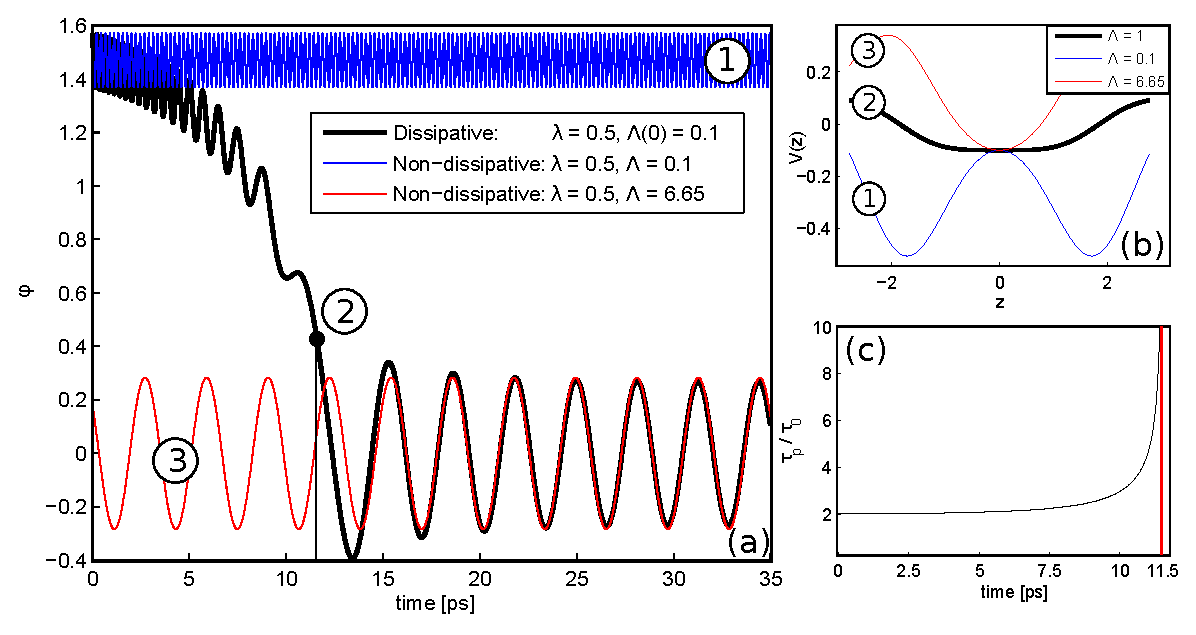
\includegraphics[width=\linewidth]{pic/phase_potential_dissipation.eps}}
\caption{(a) -- Normalized phase difference as a function of time; (b) -- effective potential vs phase parameter $z$ for red, black and blue curves, respectively, and (c) -- reduced thermon period $\tau_{p} / \tau_0$  vs time for $\kappa/\hbar = 0.1 THz$. 
Initial conditions are $S_z(0) = S_x(0) = 0$, $S_y(0) = 1$, and $\phi(0) = \pi / 2$, respectively.
\label{pic:phase}}
\end{figure}
%

Figures \ref{pic:phase}b and \ref{pic:phase}c demonstrate the suppression of $W$ -- like potential and the relevant enhancement of the reduced thermon period $\tau_{p} / \tau_0$ which occurs at $t_0 = 11.5 ps$ for  $\tau_{pol} \sim \hbar/\kappa= 10 ps$, respectively.

Thus, behavior of the phase in the presence of dissipation showed in Fig. \ref{pic:phase} is characteristic of a established non-equilibrium PT from the regime where tunneling is possible to the regime where tunneling is suppressed.
However, this regime found at $t>t_0$ cannot be interpreted immediately as the classical one.
Actually, the adiabaticity condition reads {\cite{Sols}:
%
\begin{equation}
\dfrac{1}{\omega^2(t)} \Big| \dfrac{d \omega}{d t} \Big| \ll 1.
\end{equation}
%
where $\omega(t) = B \sqrt{(1 - 2 \beta'(t))(1 - 2 \beta'(t) + 2 \alpha'(t))}/ \hbar $ is the frequency of small oscillations slowly depending on time {\cite{Sedov}. 
The solution for the phase in this case can be approximated by 
\begin{equation}
\phi(\tau) \approx \dfrac{A}{\omega(\tau)} \cos (\omega(\tau) \tau),
\end{equation}
%
where $\tau$ is the time elapsed after the oscillation sets in, and $A$ is the amplitude of oscillations at $\tau = 0$.
At large enough times, $\omega(t) \approx$ $B/ \hbar$ and permanent Rabi  oscillations for the Josephson junction phase $\phi$ are established, see Fig. \ref{pic:phase}a and Ref. {\cite{Permamemt}.
To distinguish between the quantum and classical character of these oscillations, a purely quantum approache to the problem should be considered.      
It will be in the scope of our further research.

\section*{Discussion \label{sec:conclusion}}

We have studied theoretically the coupling of two spacially separated trapped exciton polariton condensates at finite temperatures and accounting for the dissipation.
We demonstrate the crossover from thermal to quantum annealing regime for a model system of two condensates localised by a W-shape potential.
Second regime is classical one and characterizes  thermal activation.
The transition between these two regimes exhibits universal features of the 1st or 2nd order PTs which can be interpreted as PT between classical and quantum regimes. It is important that critical temperature of transition depends on some  characteristic temperature  parameter $T_{0}$ (see e.g. (\ref{eq:second_order})) that that is governed by the polariton-polariton interaction length (so-called blue shift) $\alpha N$.  It is expected that  at the temperatures sufficiently higher than  $T_{0}$ the EPJJ device operates in classical way. 

The influence of dissipation effects originating from the radiative decay of polaritons by photon tunneling through the Bragg mirrors is revealed by our analysis.
The observation of quantum tunneling processes only becomes possible within short time intervals where the dissipation cannot essentially affected to the system.
Otherwise, after some time interval the dissipation leads to crossover in the phase dynamics and it damages the W--potential as a whole, see Fig. \ref{pic:phase}.
In this case permanent Rabi  oscillations of Josephson junction phase occurs within the adiabatic approach.
To reveal either quantum of classical nature of these oscillations it is necessary to study the fluctuations of the exciton polariton system beyond the semiclassical approach represented in Sec.\ref{sec:non-equilibrium}}. 
For moderate dissipation rates and at temperatures (or relevant polariton gas densities) sufficiently below the temperature of $T_{0}$ the EPJJ device is suitable for various applications where the quantum tunneling effect is crucial. 

In order, it is quantum information processing and especially the quantum annealing problem  with exciton polariton condensates that allow for acceleration of the quantum annealing due to the final state bosonic stimulation {\cite{Yan}.
Notably the results obtained by us can be implemented here in new way.
In order, quantum tunneling effect might be utilized for design exciton polariton phase qubits similarly to superconductor devices, but in optical wavelength domain, \cite{Makhlin}.
Actually, two minima located at the points $-z_{min}$ and $+z_{max}$ of $W$-shape quantum phase potential in Fig. \ref{pic:phase_potential}b can be used for initialization of exciton polariton qubit states $\ket{0}$ and $\ket{1}$ similarly to superconductor flux qubits, respectively.
However, in our case such qubits may be tailored by external optical or electrical pump.
As a result, quantum annealing problem can be experimentally solved with help of this type of qubits \cite{Johnson}.

\section*{Methods}
\dots

% Create the reference section using BibTeX:
\bibliography{list}

\section*{Acknowledgement}
We acknowledge the financial support from RFBR, Grants No. 15-52-52001 and No. 14-02-97503.
A. Kavokin acknowledges the support from HORIZON 2020 RISE project CoExAn (Grant No. 644076) and the EPSRC Established Career fellowship on Quantum Polaritonics RP 008833.

\section*{Author contributions statement}
All authors reviewed the manuscript.

\end{document}